\begin{center}
\begin{tikzpicture}
    \node[anchor=south west,inner sep=0] (image)  at (0,0) {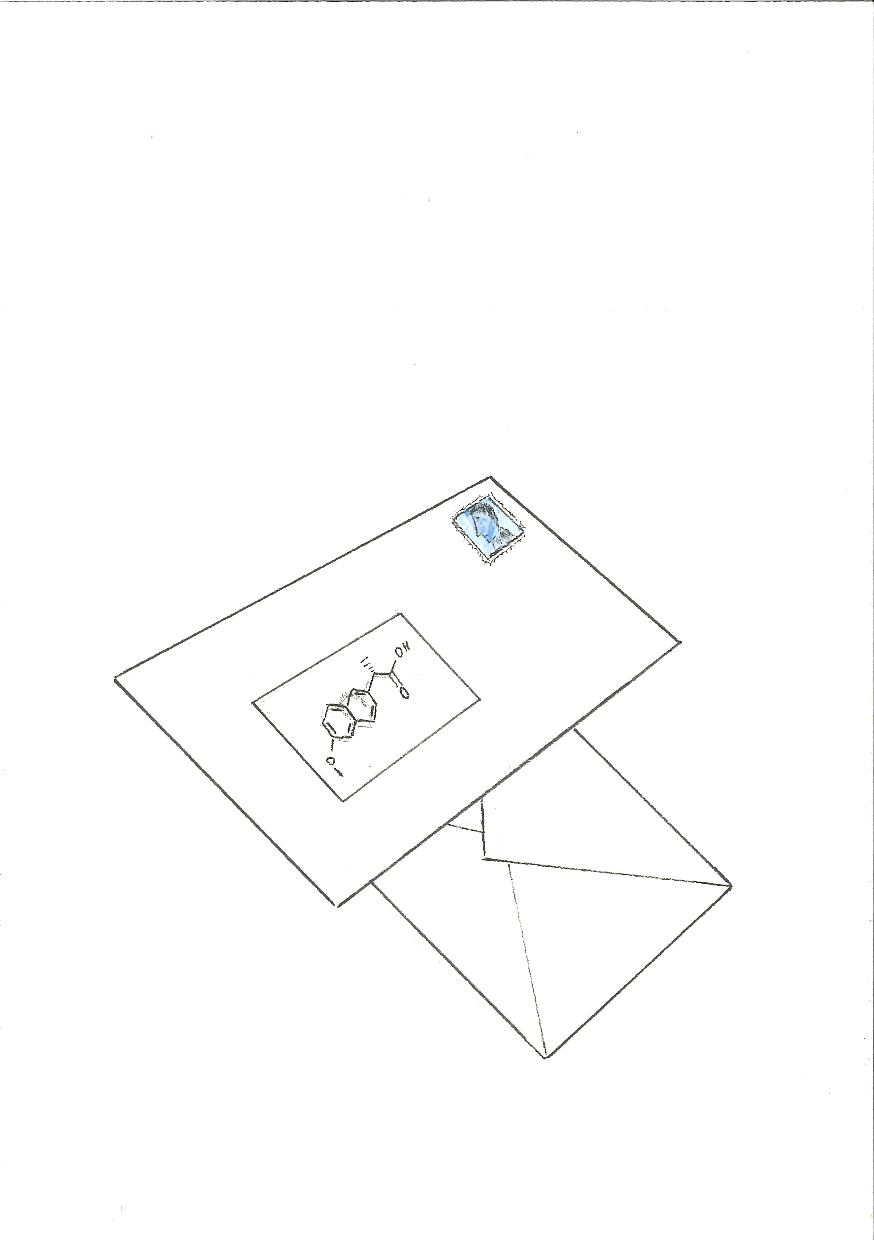
\includegraphics[trim={2mm, 2mm, 2mm, 2mm},width=0.995\pagewidth]{scans/panel-9.pdf}};
    
    
    \begin{scope}[x={(image.south east)},y={(image.north west)}]
        \if\helplines1
        	\draw[help lines,xstep=.1,ystep=.1] (0,0) grid (1,1);
        \fi
        \node[align=justify, anchor=north west, text width=6cm](en) at (0.5, 0.9) {\english{We can also block, divert, or reinforce the signals using chemical substances, that we call drugs.
        
        \doindent For example, Naproxen deactivates a protein whose taks is to send the signal of pain.}};
        
        \node[align=justify, anchor=north west, text width=6cm](es) at (0.1, 0.2) {\spanish{También podemos bloquear, redirigir, o reenforzar estas señales usando substancias químicas: lo que llamamos medicinas.}
        
        \spanish{\doindent Por ejemplo, el Naproxeno desactiva una proteína encargada de transmitir el dolor.}};
    \end{scope}
    
\end{tikzpicture}
\end{center}